% --------------------------------------------------
% This file was generated using matplottikz
% --------------------------------------------------
\documentclass[crop,tikz]{standalone}
\usepackage{tikz}
\usepackage{pgfplots}

% --------------------------------------------------
% Matplottikz color palette generated using,
%     https://www.learnui.design/tools/data-color-picker.html#palette
% --------------------------------------------------
\definecolor{matplottikz-color1}{HTML}{003f5c}
\definecolor{matplottikz-color2}{HTML}{bc5090}
\definecolor{matplottikz-color3}{HTML}{ffa600}
% --------------------------------------------------

% --------------------------------------------------
% Start of the document
% --------------------------------------------------
\begin{document}
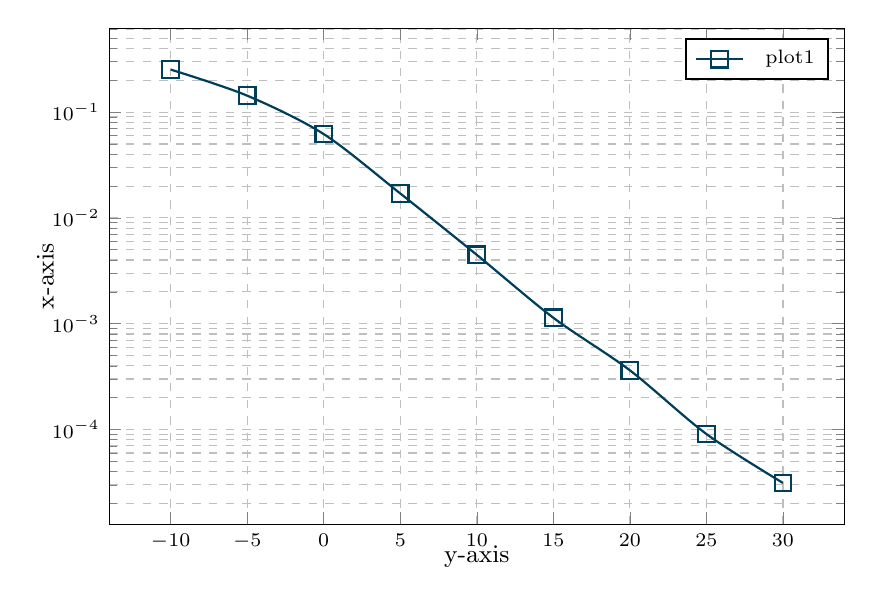
\begin{tikzpicture}
    \pgfplotsset{
        label style = {font=\fontsize{9pt}{7.2}\selectfont},
        tick label style = {font=\fontsize{7pt}{7.2}\selectfont}
    }
    \begin{axis}[
        scale = 1,
        ymode=log,
        xlabel={y-axis}, xlabel style={yshift=0.8em},
        ylabel={x-axis}, ylabel style={yshift=-0.75em},
        grid=both,
        ymajorgrids=true,
        xmajorgrids=true,
        grid style=dashed,
        width=0.9\columnwidth,
        height=0.65\columnwidth,
        legend style={
            column sep= 2mm,
            thick,
            font=\fontsize{7pt}{7.2}\selectfont,
        },
        legend columns=1,
    ]

        % -------------------------
        % Plot for: plot1
        % -------------------------
        \addplot[smooth, color=matplottikz-color1, thick, mark=square, mark size=3]
        table{
            -10 0.25239
            -5 0.14308
            0 0.061988
            5 0.017012
            10 0.004475
            15 0.0011375
            20 0.0003625
            25 9.0625e-05
            30 3.125e-05
        };
        \addlegendentry{plot1}

    \end{axis}
\end{tikzpicture}
\end{document}
% --------------------------------------------------
% End of the document
% --------------------------------------------------

% To include the figure in your latex document, use the following commands:

% \begin{figure}[!htb]
%     \centering
%     % Uncomment one of the following
%     %\includegraphics[width=0.9\columnwidth]{figures/matplottikz_logscale_example}
%     %\includestandalone[width=0.9\columnwidth]{figures/matplottikz_logscale_example}
%     \caption{Write caption here.}
%     \label{fig:matplottikz_logscale_example}
% \end{figure}
